% !TeX spellcheck = en_US
% !TeX encoding = UTF-8
% !TeX spellcheck = en_US
% !BIB TS-program = biber
% basic packages and document settings
\documentclass[a4paper,12pt]{article}
\usepackage[ngerman]{babel}
\usepackage[utf8]{inputenc}
\usepackage[T1]{fontenc}
\usepackage[a4paper]{geometry}
\geometry{top = 30mm, bottom = 25mm, left = 25mm, right = 25mm}
\usepackage{setspace}
\onehalfspacing
\raggedbottom
\pdfcompresslevel9

% mathmode-related packages
\usepackage{mathtools}
\usepackage{physics}
\usepackage{amsmath}
\usepackage{amsthm}
\usepackage{amsbsy}
\usepackage{mathrsfs}
\usepackage{amssymb}
\usepackage{amstext}
\usepackage{amsfonts}
\usepackage{tikz}
\usepackage{siunitx}
%\usepackage{IEEEtrantools}

% misc
\usepackage{esdiff}
\usepackage{multirow}
\usepackage{blindtext}
\usepackage{todonotes}
\usepackage{abstract}
\usepackage{appendix}
\usepackage[bottom]{footmisc}
\usepackage{listings}
\usepackage{dashrule}

% graphics and floats
\usepackage{graphicx}
\graphicspath{{../Figures/}}
\usepackage{tikz}
\usepackage{float}
\usepackage{wrapfig}
%\usepackage{subfloat}
\usepackage{subcaption}
%\usepackage{caption}
\usepackage[rightcaption]{sidecap}
\usepackage{tabularx}
\usepackage{adjustbox}
%\usepackage{svg}
\usepackage{epstopdf}
\usepackage{grffile}	% handle file names with dots, spaces etc.
%\usepackage{flafter}
\usepackage{rotating}
%\usepackage{floatrow}
%\floatsetup[figure]{capposition=beside,capbesideposition={top,right}}

%\usepackage{epstopdf}
%\epstopdfDeclareGraphicsRule{.pdf}{png}{.png}{convert #1 \OutputFile}
%\AppendGraphicsExtensions{.pdf}

% packages requiring setup arguments

\usepackage{xcolor}
%\definecolor{rwth-dark}{HTML}{176daf}
\definecolor{rwth-dark}{RGB}{0,84,159}
%\definecolor{rwth-light}{HTML}{8abae3}
\definecolor{rwth-light}{RGB}{142,186,229}

%/**
%* Generated by Gpick 0.2.5
%* RWTH Dark: #176daf, rgb(23, 109, 175), hsl(32, 43%, 69%)
%* RWTH Light: #8abae3, rgb(138, 186, 227), hsl(195, 73%, 89%)
%*/

\usepackage{hyperref}
\hypersetup{hidelinks=true,colorlinks=true,allcolors=rwth-dark}
\usepackage[nameinlink,capitalise]{cleveref}
%\usepackage[hyphens]{url}
%\urlstyle{sf}
%\usepackage{breakurl}


% header & footer settings
\usepackage{fancyhdr}
\pagestyle{fancy}
%\renewcommand{\chaptermark}[1]{\markboth{#1}{}} % with this we ensure that the chapter and section headings are in lowercase.
\renewcommand{\sectionmark}[1]{\markright{\thesection\ #1}}
\fancyhf{} % delete current header and footer

%\fancyhead[LE,RO]{\large\thepage}
\fancyhead[L]{\large\rightmark}
\fancyhead[R]{\large\thepage}

\renewcommand{\headrulewidth}{0.3pt}
\renewcommand{\footrulewidth}{0pt}
%\addtolength{\headheight}{0.5pt} % space for the rule

\fancyfoot[C]{\thepage}

\fancypagestyle{plain}
{
	\fancyhead{} % get rid of headers on plain pages
	\renewcommand{\headrulewidth}{0pt} % and the line
}

% ========== command definitions =================================
\newcommand{\Thickline}{\rule{\linewidth}{0.4mm}}
\newcommand{\Thinline}{\rule{\linewidth}{0.1mm}}

\newcommand{\id}{\, \mathrm{d}}

\definecolor{codegray}{gray}{0.9}
\newcommand{\code}[1]{\colorbox{codegray}{\texttt{#1}}}

\newcommand{\skippage}{\clearpage{\thispagestyle{empty}\cleardoublepage}}

\def\@esphack{%
	\relax
	\ifhmode
	\spacefactor\@savsf
	\ifdim\@savsk>\z@
	\ignorespaces
	\fi
	\fi}

\title{\LARGE title}
\date{}


\begin{document}
  
\begin{titlepage}
  \thispagestyle{empty}
  \newgeometry{top=20mm, left=20mm, right=20mm, bottom=20mm}
  
%  \begin{minipage}{0.35\textwidth}
%    \begin{flushleft}
%
%
%    \end{flushleft}
%  \end{minipage}
%  \hfill
%  \begin{minipage}{0.65\textwidth}
%    \begin{flushright}
%
%    \end{flushright}
%  \end{minipage}
  
%  \vspace*{\fill}
  \hspace{0pt}
  \vspace{2cm}
  \begin{center}
%    \Thickline
%    \vskip -0.5cm
%    \Thinline
    \hdashrule{\linewidth}{1pt}{}
    \vskip -0.5cm
    \hdashrule{\linewidth}{0.5pt}{}
    
    \vspace{0.5cm}
    \Huge{ \textbf{F17 \\}}
    \LARGE{ \textbf{Noise fundamentals} } 
    
    \hdashrule{\linewidth}{0.5pt}{}
    \vskip -0.95cm
    \hdashrule{\linewidth}{1pt}{}
%    \Thinline
%    \vskip -0.9cm
%    \Thickline 
    
    \vspace{3cm}
    \Large{\textbf{ Group 14 \\}}
    \Large{Heithem Assili, 368441 \\ Alexandre Drouet, 355095 \\ Olexiy Fedorets, 356615 \\}
    \vspace{1cm}
    \Large{\textsl{ Date of experiment: 21.03.2019 \\ Submission date: 04.04.2019}}
    
  \end{center}
  \vfill
%  \vspace*{\fill}
  
\end{titlepage}
  
  
  
%\skippage
\pagenumbering{roman}
\thispagestyle{plain}

\tableofcontents
%  \newpage
\newpage
\listoffigures

%\begingroup
%\let\cleardoublepage\relax
%\let\clearpage\relax
\listoftables
%\endgroup
%\listoftables

\skippage

\pagenumbering{arabic}
\setcounter{page}{1}
\restoregeometry
\thispagestyle{fancy}


\section{Introduction}

The goal of this experiment is to characterize and understand the effects of intrinsic thermodynamic fluctuations leading to a voltage difference across a resistor without any current applied. This is called Johnson's noise, the dependence of which on resistance, bandwidth and temperature will be analyzed. Furthermore, Boltzmann's constant will be determined from these measurements.

\subsection{Basic theoretic concepts}

Due to intrinsic thermodynamic fluctuations, the voltage $V_J$ across a resistor is fluctuating around zero even without any current applied. The mean-square of this voltage can be quantified as
\begin{equation}\label{eq:johnson-expval}
	\expval{V_J^2(t)} = 4k_B \cdot R \cdot T \cdot \Delta f
\end{equation}
From this we see that Johnson's noise is equally dependent on temperature, frequency and the actual resistance itself.

These fluctuations are very small and usually overlayed by noise from the environment or other electronics in a setup. When using an amplifier to be able to see and measure Johnson's noise, it would contribute its own rather high voltage fluctuations the total signal. However this noise can be assumed as not correlated with the Johnson's noise we would try to measure, because both are random fluctuations originating from different physical sources (resistors). This conveniently leads to the relation
\begin{equation}
	\expval{V_J^2(t) + V_N^2(t)} = \expval{V_J^2(t)} + \expval{V_N^2(t)}
\end{equation}
which is useful for calculating Johnson's noise as now the noise of the amplifier can be simply subtracted.

This leads to the formula needed to calculate the Johnson's noise mean-square $\expval{V_J^2(t)}$ from the output signal $V_{out}(t)$
\begin{equation}\label{eq:conversion}
	\expval{V_J^2(t)} = \frac{V_{out}(t) \cdot 10 \,\mathrm{V}}{G_{total}^2} - \expval{V_N^2(t)}, \quad \mathrm{with} \quad G_{total} = G_{LLE} \cdot G_{HLE}
\end{equation}
which is of course specific to our experimental setup, described in detail in \cref{sec:setup}.

We can also define the power spectral density as
\begin{equation}\label{eq:psd}
S = \expval{V_J^2(t)} / \Delta f = 4k_B \cdot R \cdot T \cdot
\end{equation}
which is in this case a factor of $R$ away from actual power ($P = U^2/R$). Johnson's noise is usually approximated as white, meaning that the power spectral density is constant over the frequency spectrum.

\subsection{Experimental setup} \label{sec:setup}

The setup for this experiments consist of two main parts: the low-level and high-level electronics. 

The low-level electronics basically resemble two op-amps with variable input and feedback resistors. They give a total gain of $G_{LLE} = 5100$.

The high-level electronics consist of multiple stages which are wired one after the other. These are a high-pass and low-pass filter with variable cutoff frequencies $f_1$ and $f_2$, an amplifier with variable gain $G_{HLE}$, and a multiplier. There is also an output module for time averaging of the signal, which we will only use for self-control and not for the actual measurements, because it is not very reliable and exact.

Additionally, we will need an arbitrary waveform generator (AWG) to input a known signal necessary for some characterization measurements, and of course an oscilloscope to visualize and measure properties of signals.

For the measurement at low temperature, we use two resistors submerged into liquid nitrogen.

\section{Setup characterization measurements}

For the error calculation in the following and all further analysis we will use the Python package \code{uncertainties}\footnote{\url{https://pythonhosted.org/uncertainties/user_guide.html}}, which implements numerical calculations of Gaussian error propagation using automatic differentiation methods.

\subsection{Measurements of actual amplifier gain}

Because amplification is never perfect, we need to first measure the actual gains for different settings of the amplifier module. We record input and output voltage RMS values using the oscilloscope, for which we assume errors of 0.2 mV and 10 mV, respectively.

To verify the $\pm 10$ V range of the high-level electronics we also record the clipping voltage for the first three gain settings, which was 10.1 V, 9.6 V and 9.9 V.

\begin{table}[H]
	\renewcommand{\arraystretch}{1}
	\centering
%	\large
%	\begin{adjustbox}{width=\textwidth}
		\begin{tabular}{|c|c|}
			\hline
			Set gain & Measured gain \\
			\hline
			$10.0$ & $9.94 \pm 0.01$ \\
			\hline
			$15.0$ & $14.84 \pm 0.02$ \\
			\hline
			$20.0$ & $19.58 \pm 0.03$ \\
			\hline
			$30.0$ & $29.22 \pm 0.04$ \\
			\hline
			$40.0$ & $38.24 \pm 0.08$ \\
			\hline
			$50.0$ & $48.09 \pm 0.08$ \\
			\hline
			$60.0$ & $61.3 \pm 0.1$ \\
			\hline
			$80.0$ & $61.6 \pm 0.1$ \\
			\hline
			$100.0$ & $101.2 \pm 0.2$ \\
			\hline
			$100.0$ & $99.3 \pm 0.2$ \\
			\hline
			$150.0$ & $147.3 \pm 0.5$ \\
			\hline
			$200.0$ & $197.4 \pm 0.6$ \\
			\hline
			$300.0$ & $33.2 \pm 0.3$ \\
			\hline
			$400.0$ & $406 \pm 13$ \\
			\hline
			$500.0$ & $491 \pm 15$ \\
			\hline
			$600.0$ & $594 \pm 18$ \\
			\hline
			$800.0$ & $788 \pm 23$ \\
			\hline
			$1000.0$ & $988 \pm 29$ \\
			\hline
			$1000.0$ & $985 \pm 29$ \\
			\hline
			$1500.0$ & $1479 \pm 44$ \\
			\hline
			$2000.0$ & $1968 \pm 58$ \\ 
			$3000.0$ & $2654 \pm 200$ \\
			\hline
			$4000.0$ & $3977 \pm 306$ \\
			\hline
			$5000.0$ & $4992 \pm 384$ \\
			\hline
			$6000.0$ & $5992 \pm 461$ \\
			\hline
			$8000.0$ & $7638 \pm 588$ \\
			\hline
			$10000.0$ & $8231 \pm 633$ \\
			\hline
		\end{tabular}
%	\end{adjustbox}
	\caption{Set and measured gains of the amplifier. Multiple values for the same set gain mean that it was set using different settings of the stages within the amplifier, as for example $100 \equiv 10 \times 1 \times 10 \equiv 1 \times 10 \times 10$.}
	\label{tab:gains}
\end{table}


\subsection{Multiplier module}

By using the XY (CH1 vs CH2) mode of the oscilloscope, we can verify the operation of the multiplier module operating as a squarer. In \cref{fig:amplifier-base} we see a parabola as expected. Additionally, with increasing input frequency we start seeing deviations from the parabolic shape, until we arrive at the so-called Lissajous-curve for a frequency ratio of 1:2 in \cref{fig:amplifier-lissajous}. After that, the parabola flips.

We were not able to find any limit to the input voltage or frequency for the amplifier module within the boundaries given by the AWG.

\begin{figure}[H]
	\centering
	\begin{subfigure}{0.49\textwidth}
		\centering
		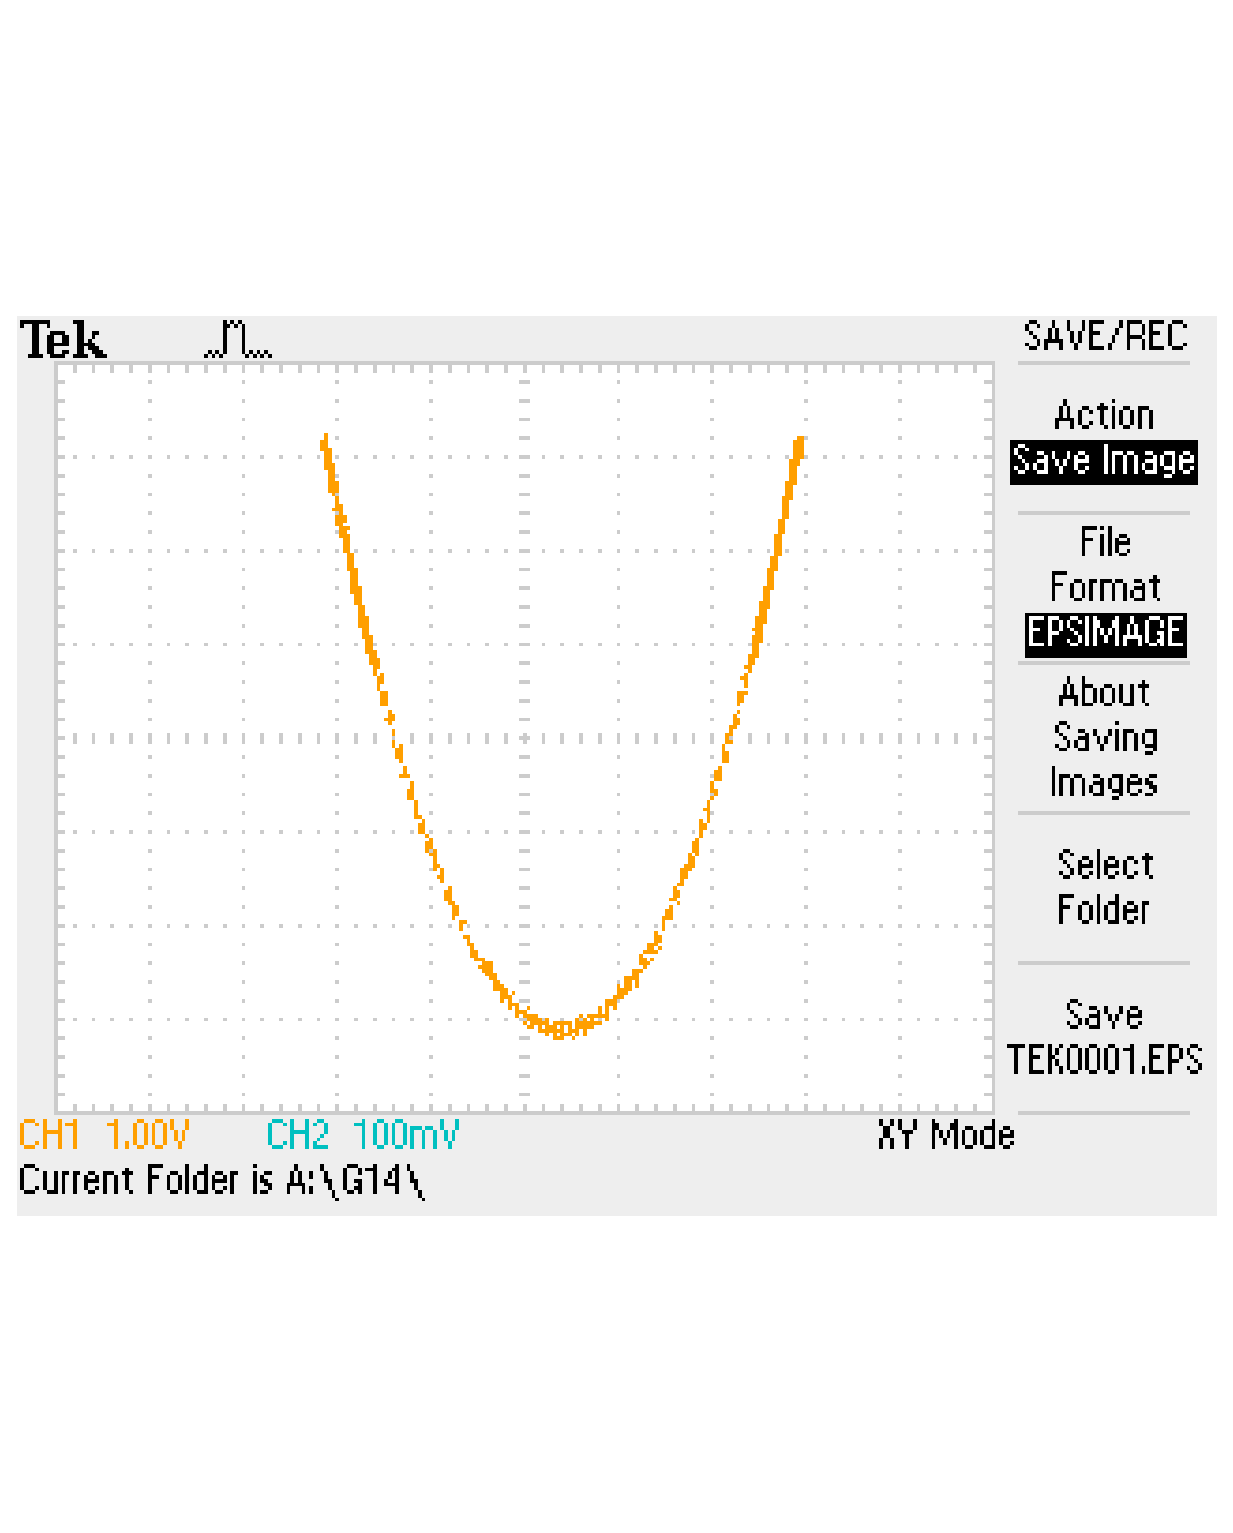
\includegraphics[width=\textwidth,clip,trim={0 5cm 3.4cm 5cm}]{TEK1.eps}
		\caption{}
		\label{fig:amplifier-base}
	\end{subfigure}
	\begin{subfigure}{0.49\textwidth}
		\centering
		\includegraphics[width=\textwidth,clip,trim={0 5cm 3.4cm 5cm}]{TEK2.eps}
		\caption{}
	\end{subfigure}
%	\vskip 10pt
	\begin{subfigure}{0.49\textwidth}
		\centering
		\includegraphics[width=\textwidth,clip,trim={0 5cm 3.4cm 5cm}]{TEK3.eps}
		\caption{}
		\label{fig:amplifier-lissajous}
	\end{subfigure}
	\begin{subfigure}{0.49\textwidth}
		\centering
		\includegraphics[width=\textwidth,clip,trim={0 5cm 3.4cm 5cm}]{TEK4.eps}
		\caption{}
	\end{subfigure}
	
	\caption{Screenshots of the oscilloscope using the XY-mode. Frequency difference between the channels is increasing from (a) to (d).}
	\label{fig:xy}
\end{figure}


\subsection{Bandpass filter}
\subsubsection{Phase response}

We analyze the phase response of our bandpass filter by varying the input frequency and measuring the phase difference between input and output channels using the corresponding oscilloscope function. We observe that phase difference is changing from positive to negative with increasing frequency, as can be seen in \cref{fig:phase}. This linear behavior around a center frequency is expected from a passive bandpass filter, see \cref{fig:fil.png}.

\begin{figure}[H]
	\centering
	\begin{subfigure}{0.49\textwidth}
		\centering
		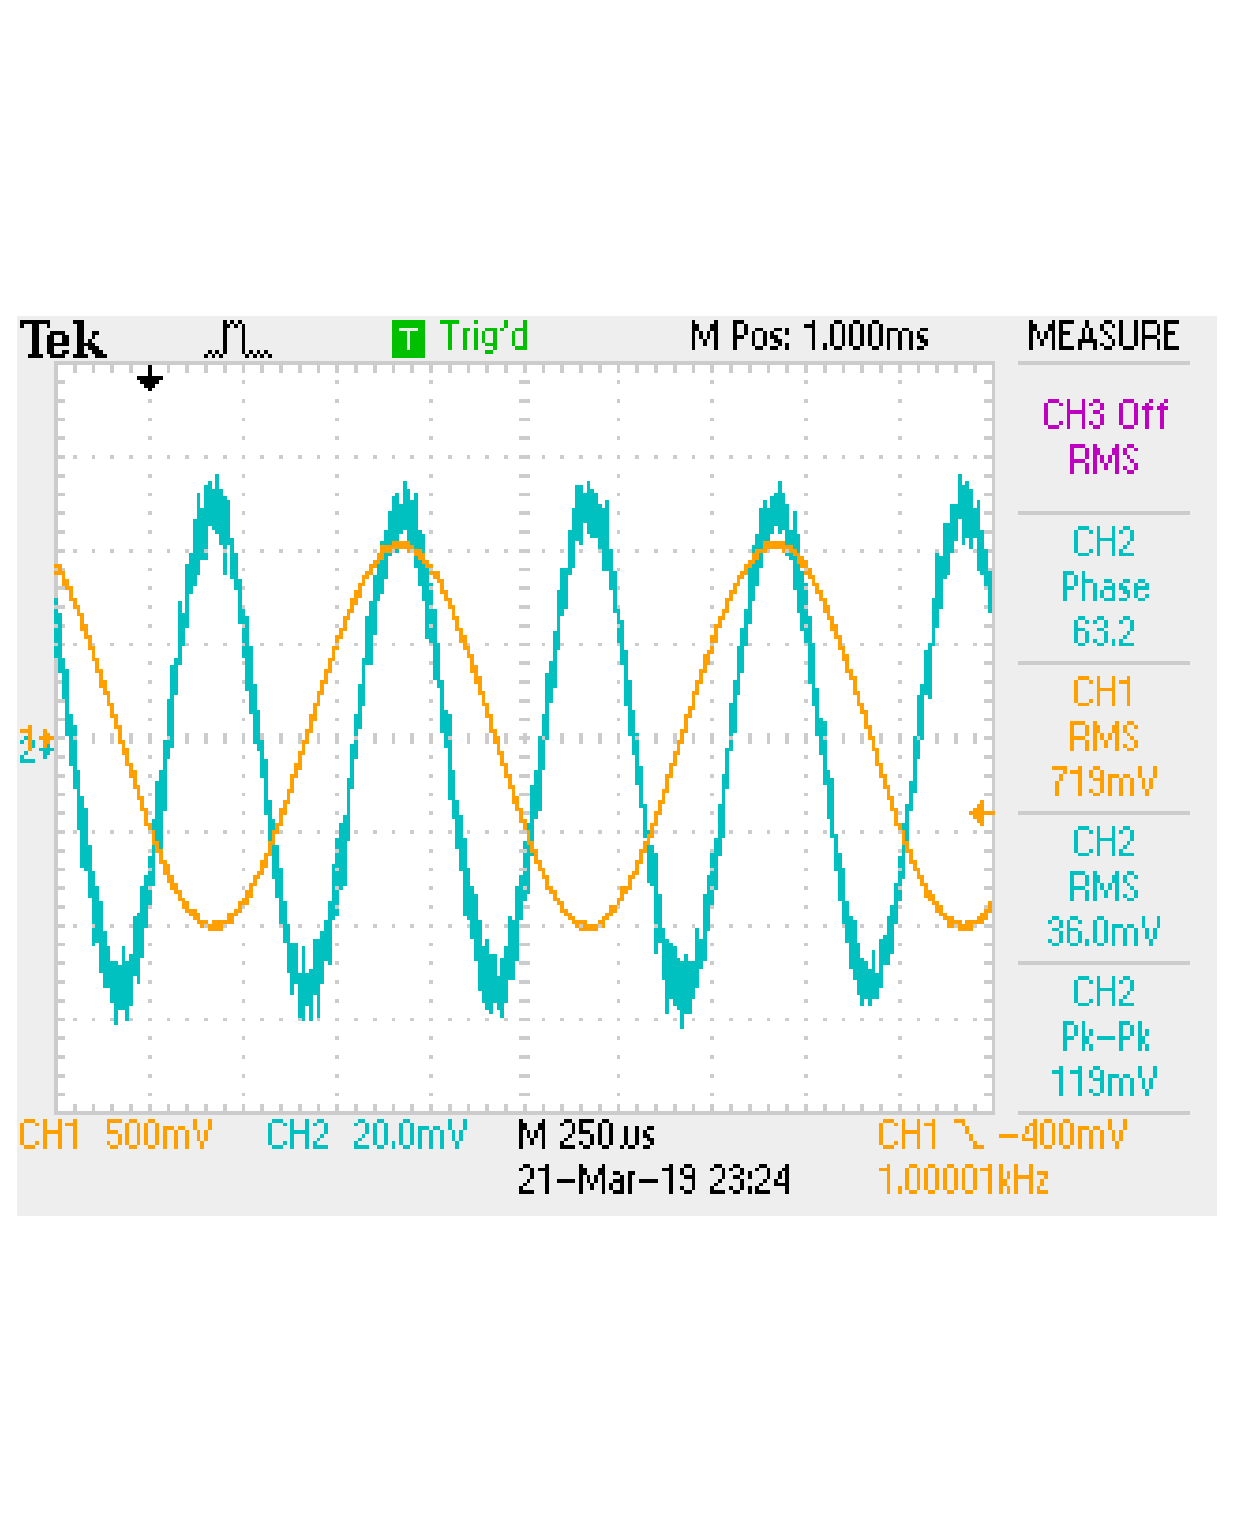
\includegraphics[width=\textwidth,clip,trim={0 5cm 0 5cm}]{F0002TEK.eps}
		\caption{}
	\end{subfigure}
	\begin{subfigure}{0.49\textwidth}
		\centering
		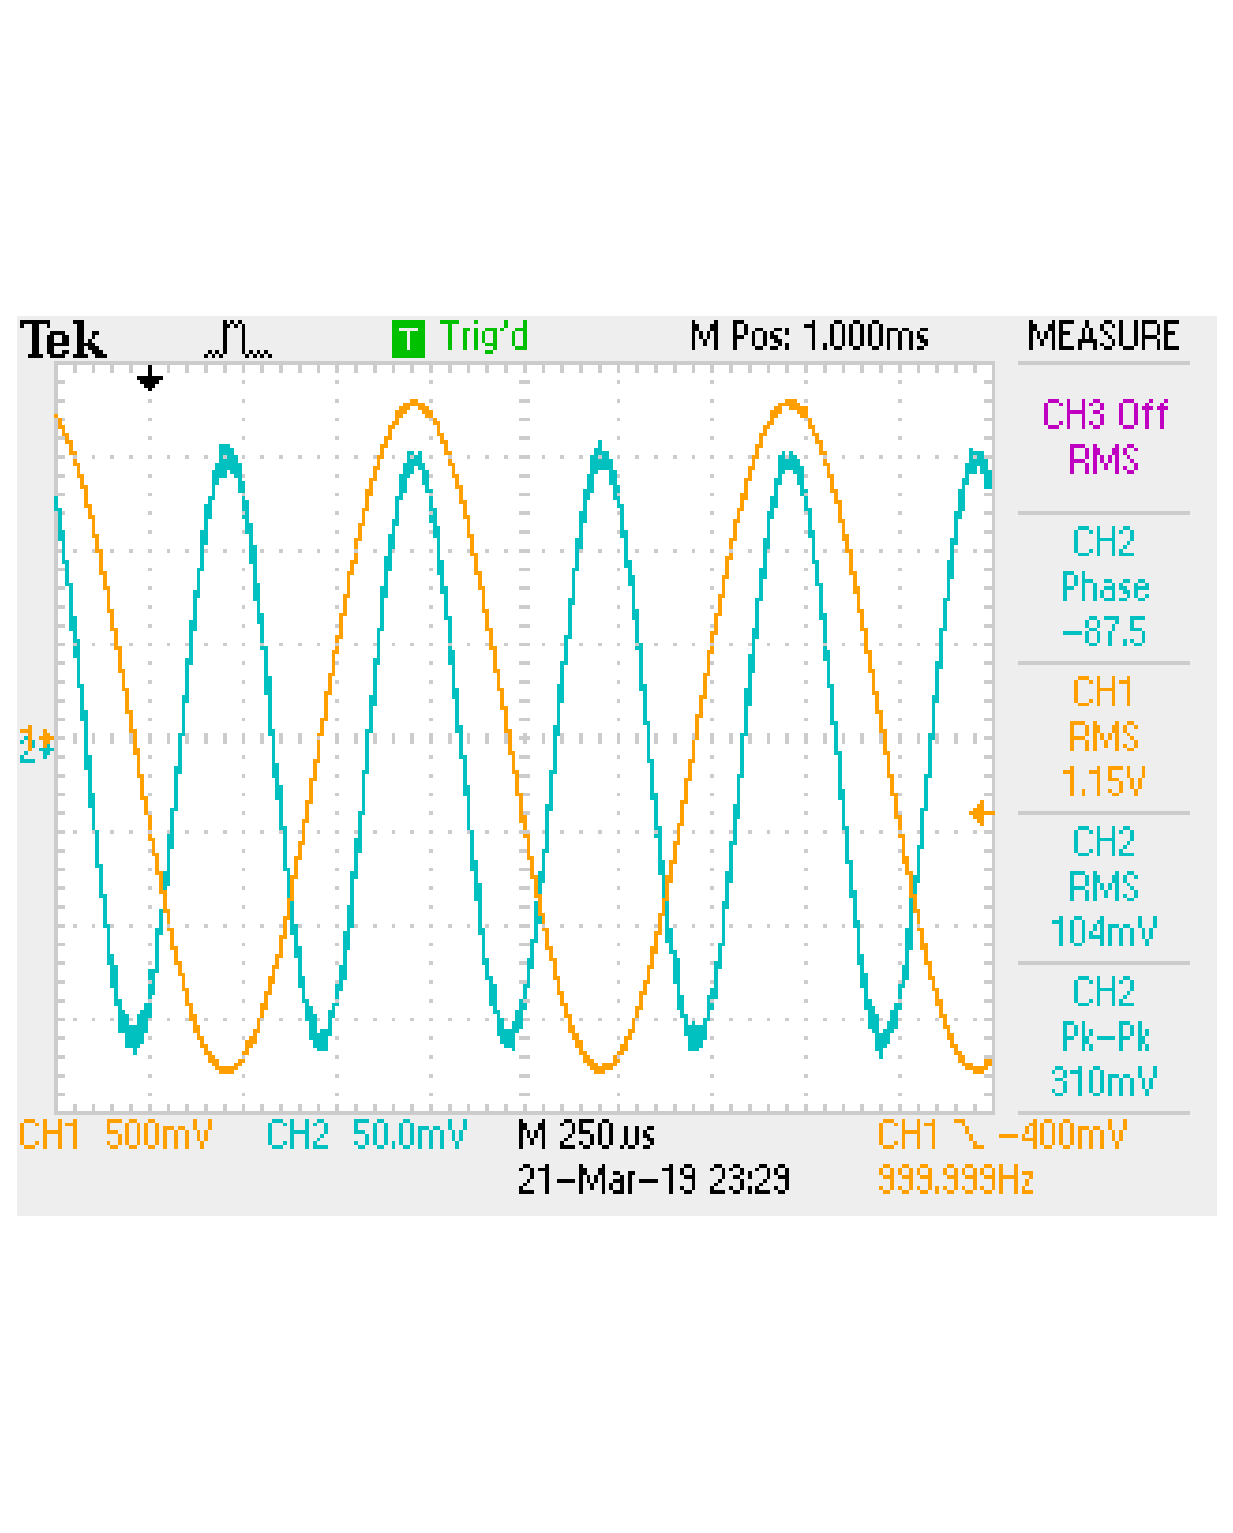
\includegraphics[width=\textwidth,clip,trim={0 5cm 0 5cm}]{F0005TEK.eps}
		\caption{}
	\end{subfigure}
	
	\caption{Screenshots of the oscilloscope in phase measuring mode, for different input frequency. }
	\label{fig:phase}
\end{figure}

\begin{figure}[H]
	\centering
	\includegraphics[width=0.8\textwidth]{fil.png}
	\caption{Phase response of a passive bandpass filter.\protect\footnotemark}
	\label{fig:fil.png}
\end{figure}
\footnotetext{Image taken from \url{https://www.electronics-tutorials.ws/filter/filter_4.html}.}

\subsubsection{Gain dependence on frequency}

To verify the operation of the low- and high-pass filter system within the high-level electronics module, we measure the output voltage and compute the gain for a large range of frequencies, adjusting the sampling rate to the slope. The cutoff frequencies are set to $f_1 = 1 \,\mathrm{kHz}$ and $f_2 = 10 \,\mathrm{kHz}$ and the input voltage is fixed at $V_{in} = (106 \pm 0.5) \,\mathrm{mV}$. We estimated this error and the assumed $\pm 0.01$ mV on the output via observing the fluctuations of the signal on the oscilloscope.

We can now compute the actual cutoffs at the -3 dB threshold corresponding to a $1/\sqrt{2}$ fraction of the maximum gain, which indeed turn out to be at exactly 1 kHz and 10 kHz (of course only as far as our resolution in frequency at these regions allows).

Besides that, it is remarkable that the response of the filter is not symmetric and that the gain varies significantly within the passing band, indicating a highly non-perfect filter.

\begin{figure}[H]
	\centering
	\includegraphics[width=\textwidth]{Bandpass_GainVsFrequency_4b.pdf}
	\caption{Frequency response of the bandpass filter, with cutoff frequencies at -3 dB relative to maximum gain. Errorbars are too small to be visible here.}
	\label{fig:Bandpass_GainVsFrequency_4b.pdf}
\end{figure}



\clearpage
\section{Johnson's noise \& Boltzmann's constant}

\subsection{Room temperature measurement}\label{sec:RT}

\subsubsection{Dependence on resistance}\label{eq:VJ-vs-R}

We set the bandwidth fixed to 9 kHz ($f_1 = 1 \,\mathrm{kHz}, \, f_2 = 10 \,\mathrm{kHz}$) and vary the input resistance in the low-level electronics over a large range. We adjust the gain of the HLE-amplifier such that the output of the multiplier module does not exceed 1 V. For each resistance, we record three values of the output to be able to calculate the mean with error $\sigma/\sqrt{3}$.

We also measured the room temperature to be $T_{RT} = 294.4 \pm 0.1 \,\mathrm{K}$.


\begin{figure}[H]
	\centering
	\includegraphics[width=\textwidth]{Johnson-NoiseVsResistance.pdf}
	\caption{Linear fits, excluding the last point, to find the amplifier noise (green) and calculate Boltzmann's constant (magenta). Values for Johnson noise at lower resistances are not fully depicted due to the fact that negative values (errorbars) can not be shown on a log-plot. Lower plot shows residuals, note the linear y-axis.}
	\label{fig:Johnson-NoiseVsResistance.pdf}
\end{figure}

We can now fit a linear model $f(R) = a \cdot R + b$ to the data, excluding the last point at very high resistance, which we classified as an outlier possibly indicating a change at high resistances, as it does not correspond with the others. This yields the amplifier noise $\expval{V_N^2(t)}$ at $R=0$ as the parameter $b$. Using \cref{eq:conversion} and values for the actual gain from \cref{tab:gains}, corresponding to the one we set at the amplifier, we can now calculate the Johnson noise amplitude $\expval{V_J^2(t)}$ which we are interested in.

The results of this procedure are shown in \cref{fig:Johnson-NoiseVsResistance.pdf}. It is notable that errors get very large for Johnson noise at low resistances, probably resulting in the value of $b$ to correspond with zero within its error. The value of $\chi^2/ndf$ turn out to be acceptable when excluding the last point.

Using the fit results of the corrected noise amplitude and \cref{eq:johnson-expval}, we can calculate Boltzmann's constant
\begin{equation}
	k_B = \frac{a}{4 \cdot T_{RT} \cdot \Delta f} = (2.09 \pm 0.08) \times 10^{-23} \SI{}{J/K}
\end{equation} 
which lies $\approx 8.6 \,\sigma$ away from the true value of $1.3806503 \times 10^{-23} \SI{}{J/K}$.

\subsubsection{Dependence on bandwidth}

Analogously to the previous section we can measure the dependence of Johnson's noise on bandwidth (frequency). We therefore keep $R_{in} = 10 \,\mathrm{k}\Omega$ fixed and vary the bandwidth over predefined values of $f_1$ and $f_2$. 

Because the amplifier noise may also depend on frequency, we measure it for each bandwidth setting using $R_{in} = 10 \,\Omega$ as an approximation to zero resistance. We subtract it from each measurement to come closer to the true Johnson noise $\expval{V_J^2(t)}$.

Despite the larger errors, the exclusion of points at high bandwidth from the fit is less justified. It improved only $\chi^2/ndf$ but not the value of $k_B$. \cref{fig:Johnson-NoiseVsBandwidth_RT.pdf} shows the fit including all the measured values.


Similar to above, the fit yields a value for Boltzmann's constant of
\begin{equation}
k_B = \frac{a}{4 \cdot T_{RT} \cdot R} = (2.00 \pm 0.08) \times 10^{-23} \SI{}{J/K}
\end{equation}
which lies $\approx 7.7 \,\sigma$ away from the true value. 


Additionally, we can plot Johnson noise against the equivalent noise bandwidth, which is shown in \cref{fig:Johnson-NoiseVsENBW_RT.pdf} \footnote{Values for the ENBW were used as given in the instruction manual.}. Here we can see a clear linear dependence of $\expval{V_J^2(t)}$ on the ENBW.

\begin{figure}[H]
	\centering
	\includegraphics[width=0.95\textwidth]{Johnson-NoiseVsBandwidth_RT.pdf}
	\caption{Linear fit to the corrected noise amplitude, no points are excluded. Lower plot shows residuals, note the linear y-axis.}
	\label{fig:Johnson-NoiseVsBandwidth_RT.pdf}
\end{figure}


\begin{figure}[H]
	\centering
	\includegraphics[width=0.75\textwidth]{Johnson-NoiseVsENBW_RT.pdf}
	\caption{Johnson noise plotted over equivalent noise bandwidth, showing a clear linear behavior. Errors on the ENBW were given as 4\%.}
	\label{fig:Johnson-NoiseVsENBW_RT.pdf}
\end{figure}

Lastly, we calculate the power spectral density of Johnson's noise using \cref{eq:psd}. It appears to be randomly fluctuating around a mean, as it would be expected from a white noise characteristic.

For reference, the values of the PSD expected from computed and true $k_B$-values are shown as horizontal lines. Of course the value from the computed $k_B$ corresponds perfectly as expected, coming from the same dataset. Using the true $k_B$-value we see that the PSD amplitude would be expected much lower. This indicates an overestimation of $\expval{V_J^2(t)}$.

\begin{figure}[H]
	\centering
	\includegraphics[width=\textwidth]{Johnson-NoisePSD_RT.pdf}
	\caption{The power spectral density of the measured Johnson noise. It looks like random fluctuations around a mean, which would be expected from white noise. Expected PSD amplitudes are shown as horizontal lines.}
	\label{fig:Johnson-NoisePSD_RT.pdf}
\end{figure}



\subsection{Measurement at $T_{N_2}=77 \, \mathrm{K}$}

Analogously to \cref{sec:RT}, we perform measurements of noise dependence on bandwidth using resistors at the boiling temperature of liquid nitrogen $T_{N_2}=77 \, \mathrm{K}$. The values of those were measured to $R_A = 9.7 \,\Omega$ and $R_B = 9.99 \,\mathrm{k}\Omega$.

Similar to the above, the fit to the corrected Johnson noise mean-square $\expval{V_J^2(t)}$ yields a value for Boltzmann's constant of
\begin{equation}
k_B = \frac{a}{4 \cdot T_{N_2} \cdot R_B} = (2.80 \pm 0.20) \times 10^{-23} \SI{}{J/K}
\end{equation}
which lies $\approx 7.1 \,\sigma$ away from the true value.

\begin{figure}[H]
	\centering
	\includegraphics[width=\textwidth]{Johnson-NoiseVsBandwidth_77K.pdf}
	\caption{Linear fit to the corrected noise amplitude, no points are excluded. Lower plot shows residuals, note the linear y-axis.}
	\label{fig:Johnson-NoiseVsBandwidth_77K.pdf}
\end{figure}

\begin{figure}[H]
	\centering
	\includegraphics[width=\textwidth]{Johnson-NoiseVsENBW_77K.pdf}
	\caption{Johnson noise plotted over equivalent noise bandwidth, showing a less linear behavior than \cref{fig:Johnson-NoiseVsENBW_RT.pdf}. Errors on the ENBW were given as 4\%.}
	\label{fig:Johnson-NoiseVsENBW_77K.pdf}
\end{figure}

In contrast to \cref{fig:Johnson-NoiseVsENBW_RT.pdf}, the noise over ENBW at $T_{N_2}$ is less clear linear and shows an outlier at $\approx 10^4$ Hz, which could is expected from the data in \cref{fig:Johnson-NoiseVsBandwidth_77K.pdf}.

The power spectral density at cold temperature, shown in \cref{fig:Johnson-NoisePSD_77K.pdf}, yields similar conclusions to what was seen in the results at room temperature (\cref{fig:Johnson-NoisePSD_RT.pdf}). Although the difference to the noise levels expected from the true $k_B$ is much less. the amplitude of the fluctuations of the PSD is approximately the same as for room temperature $(\approx 1 \times 10^{-16} \,\mathrm{V}^2/\mathrm{Hz} )$.


\begin{figure}[H]
	\centering
	\includegraphics[width=\textwidth]{Johnson-NoisePSD_77K.pdf}
	\caption{The power spectral density of the measured Johnson noise.  Expected PSD amplitudes are shown as horizontal lines. The result is similar to \cref{fig:Johnson-NoisePSD_RT.pdf}.}
	\label{fig:Johnson-NoisePSD_77K.pdf}
\end{figure}



\clearpage
\section{Conclusion}

\begin{table}[H]
	\renewcommand{\arraystretch}{1.5}
	\centering
	\Large
	\begin{adjustbox}{width=1\textwidth}
		\begin{tabular}{c|ccc}
			& from R-dependence & from $\Delta f$-dependence at RT & from $\Delta f$-dependence at 77 K 
			\\
			\hline
			$k_B \, (\SI{}{J/K})$ & $(2.09 \pm 0.08) \times 10^{-23}$ & $(2.0 \pm 0.08) \times 10^{-23}$  & $(2.80 \pm 0.20) \times 10^{-23}$
			\\
			Deviation & $8.6 \, \sigma$ & $7.6 \, \sigma$ & $7.1 \, \sigma$
			\\
		\end{tabular}
	\end{adjustbox}
	\caption{A compilation of all calculated values of the Boltzmann-constant }
	\label{tab:kB}
\end{table}

Over the course of the experiment, we were able to familiarize with the electronic components and detect Johnson's noise of an amplitude up to and below $10^{-13}$ Volt. Its white noise nature could be indicated through the power spectral density.

The calculated values of Boltzmann's constant all lie significantly above the true value. As can also be seen from plots of the power spectral density, this indicates that we overestimate the Johnson noise amplitude $\expval{V_J^2}$. A reason for this can be that we neglected electrostatic, electromagnetic and vibrational coupling of the components to the environment. The effect of these would have to be subtracted (similar to how we dealt with the amplifier noise $\expval{V_N^2}$), to get closer to the true value of $k_B$. It is, however, not straightforward to estimate the extent of those effects.


\end{document}
